
\documentclass{article}
\usepackage[english]{babel}
\usepackage[utf8]{inputenc}
\usepackage{tikz}
\usepackage{graphicx}
\usepackage{float}
\usepackage{longtable}
\usepackage{booktabs}
\usepackage{caption}




\title{RASDproj}

\date{Prof. Elisabetta Di Nitto  -  Anno 2021/2022}

\author{Sofia Martellozzo - 
      Valeria Detomas 
}

\begin{document}
\maketitle
\newpage
\renewcommand\contentsname{Contents}
\tableofcontents

\newpage

\section{Introduction}

\subsection{Purpose}
The purpose of this document is to thoroughly describe 
Data-dRiven PrEdictive FArMing in Telengana(DREAM).
It presents functional and non functional requirements of the system and its components.
Moreover it provides use cases and scenarios for the users involved.
\\This document is meant as a contractual basis for the customer and the developer.

\subsubsection{Goals}
\label{section:1.1.1}
\begin{itemize}
    \item  allow policy makers to retrieve information from farmers
\item allow farmers to communicate with each other
\item allow farmers to insert data, questions, problems
\item the impact of meteorological data on farmers activity can be used for further information
\item allow farmers to retrieve information relevant for their activity (meteo, humidity..)
\end{itemize}

\subsection{Scope}
The aim of the system is to acquire and combine data and 
information of farmers in Telengana. 
The system will also provide support both to Telengana's 
policy makers and farmers thanks to 
new innovative technologies.
\\
(non so se vogliamo mettere questo : The system consists in a back-end server application and in a web application front-end)
\\
Thanks to the system policy makers are able to get a complete picture of the agriculture status in the whole state.
    In order to do this,  Dreams provides information that makes them able to give incentives to those farmers who are performing well and keep track of those who needs help.
    The farmers have access to a forum on which they are able to communicate with other farmers, a forum to spread useful suggestions and to request for help to those who are having a harder time.
    The application provides a personalized page for each farmer in which they can find, based on his location and type of production, specific advice, meteorological forecasts and the condition of the soil.
    This information are already provided by Telengana's government.
    In this page they can also find several buttons, one that allows them to specify any problem that they face,
    another one to update their production trend. There is also another button to let those who are recognized as good farmers send advice to the system, so that everyone can improve their knowledge about the local farming ...
    Data concerning weather are already provided by Telengana's government,

\subsubsection{world phenomena}
\begin{itemize}
    \item farmers decide type of production
    \item weather conditions influence production
    \item agronomists visit periodically farmers
    \item agronomists respond to help requests from farmers
    \item farmers can be identified as those who are performing well or not.
    \item farmers receive some type of advantage if they are the best one in their production activity
\end{itemize}

\subsubsection{shared phenomena}

\begin{itemize}
    \item humidity of soil is measured by sensors 
    \item amount of water used by each farmer is retrieved by water irrigation system
    \item Telengana's governments collects data concerning weather forecast
    \item farmers insert data about their production in the system
    \item farmers can insert problems they face into the system
    \item farmers can answer to requests for help from other farmers
    \item farmers can discuss with each other through the system
    \item the system identifies the farmers who are performing well
\end{itemize}

\subsection{Glossary}
\subsubsection{Definitions}
\subsubsection{Acronyms}
\subsubsection{Abbreviations}






\section{Overall Description}
\subsection{Product Perspective}
\subsubsection{Class Diagram}
\begin{figure}[H]
    \begin{center}
    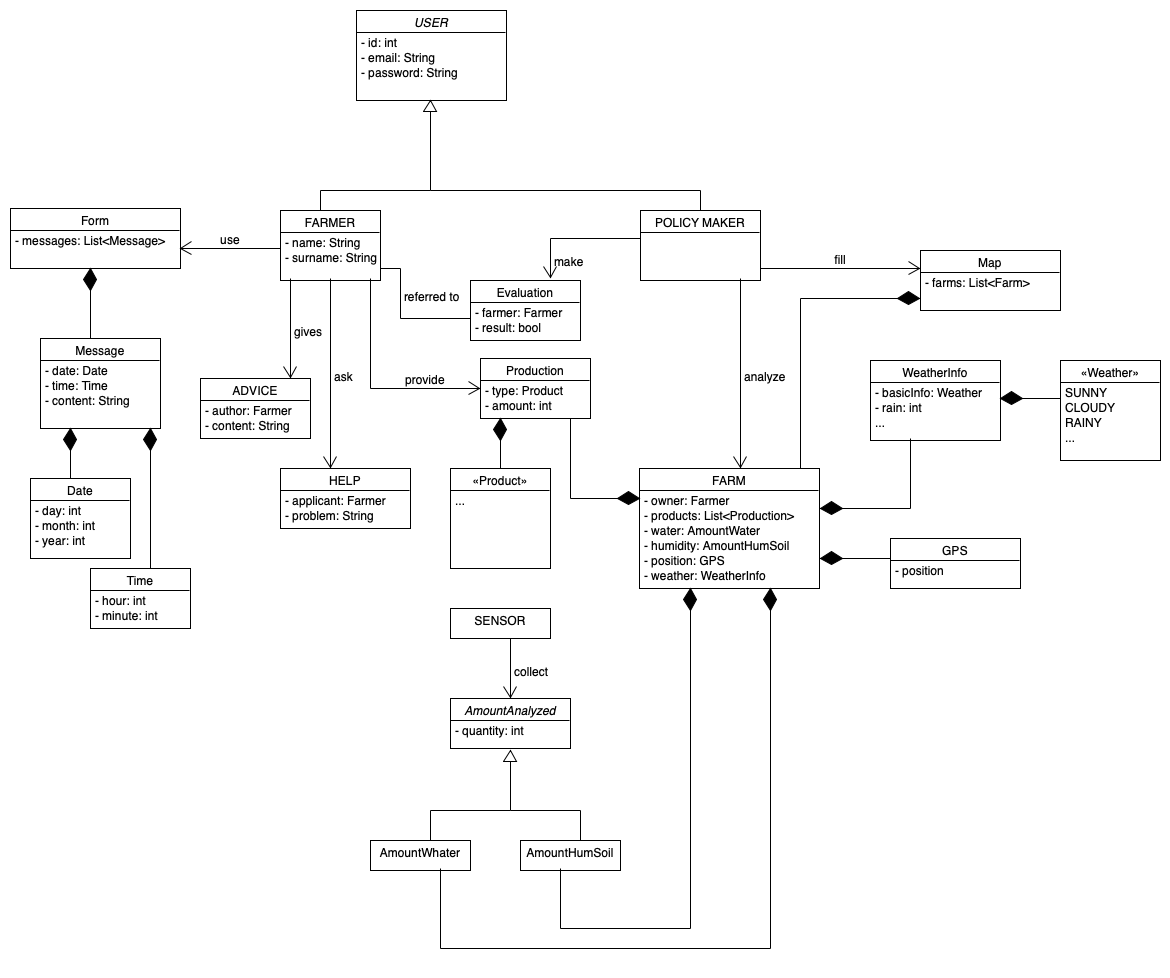
\includegraphics[width=1\textwidth]{images/UMLSW2_1.png}
    \caption{UML diagram.}
    \label{fig:uml}
    \end{center}
\end{figure}
\subsubsection{State Diagram}
\begin{figure}[H]
    \begin{center}
    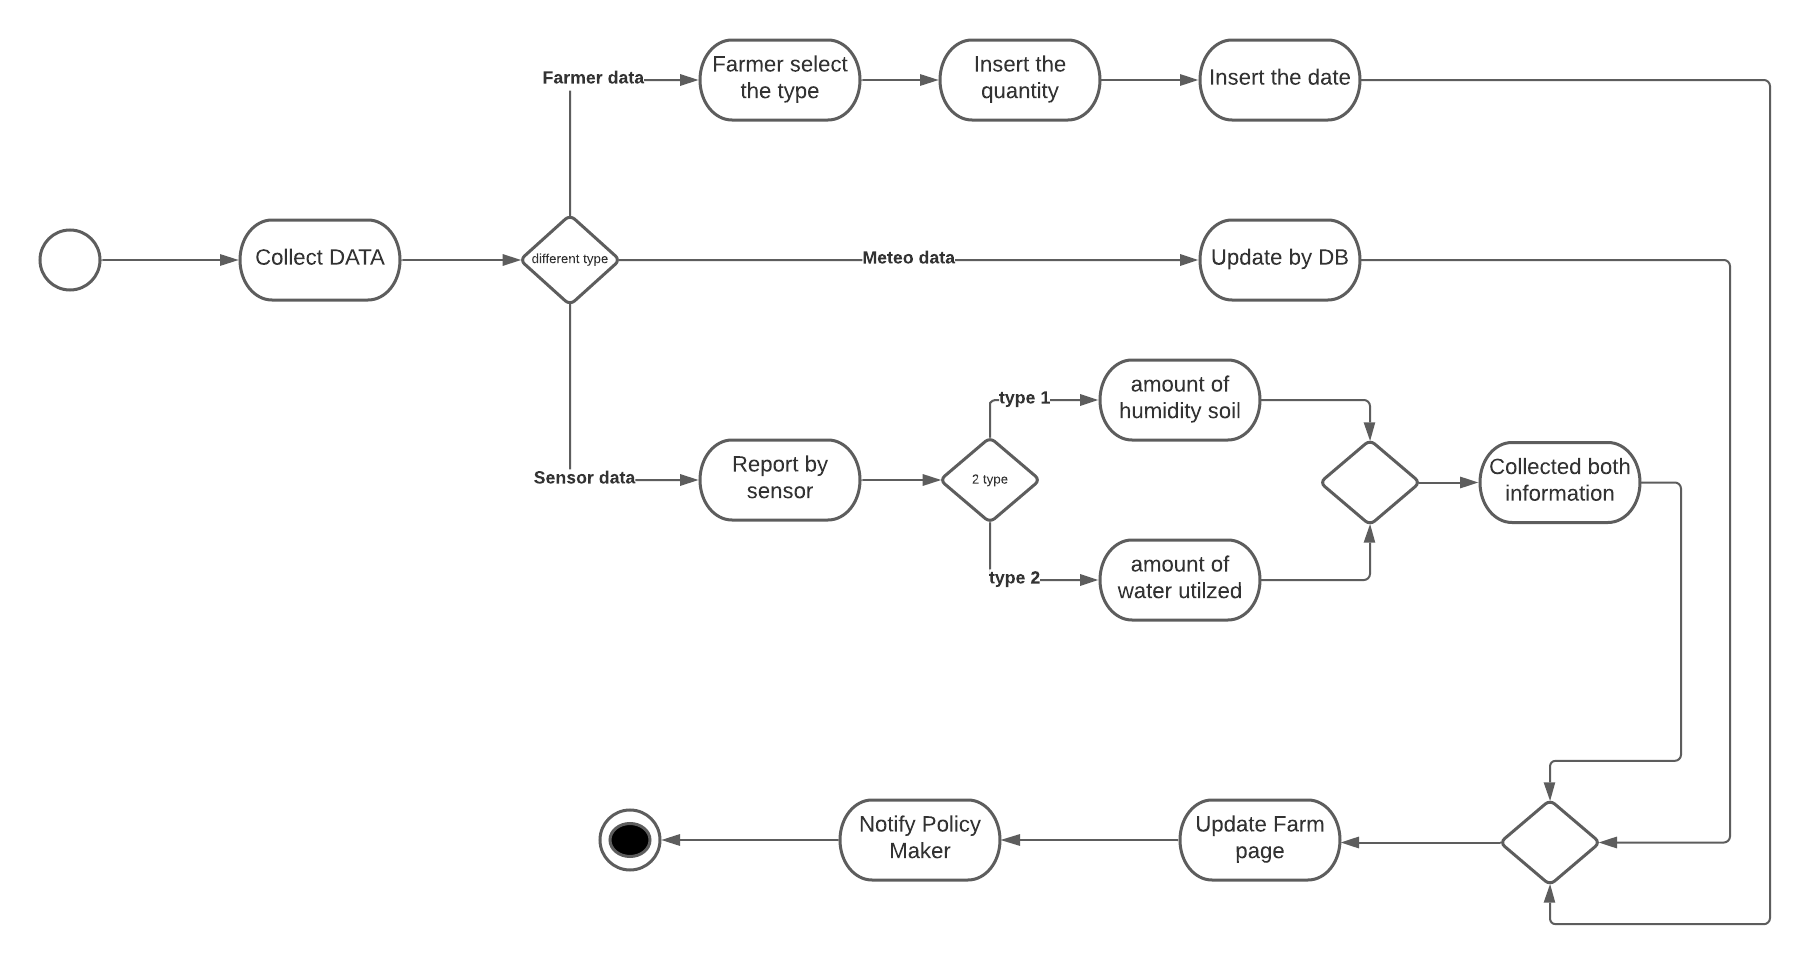
\includegraphics[width=1\textwidth]{images/State chart 1.png}
    \caption{Update Farmer page.}
    \label{fig:state1}
    \end{center}
\end{figure}
\begin{figure}[H]
    \begin{center}
    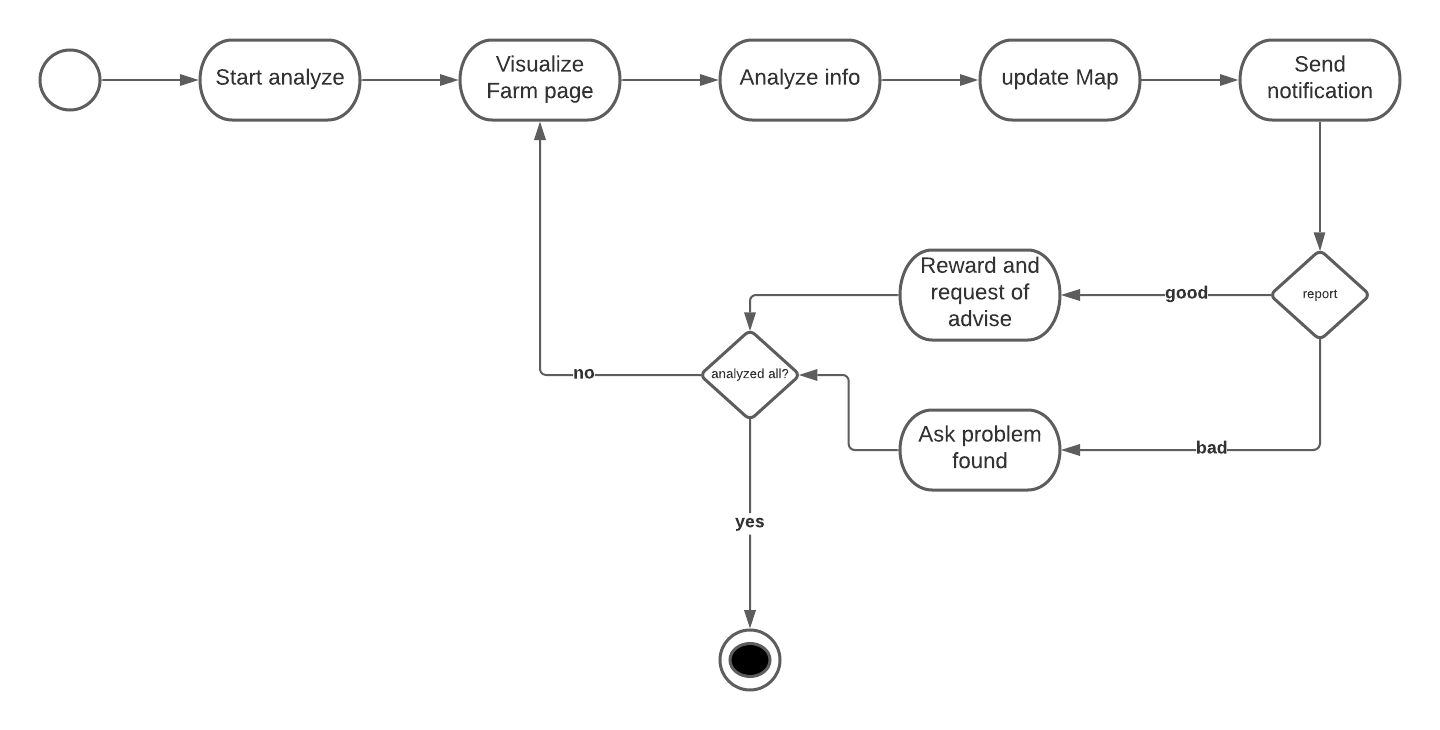
\includegraphics[width=1\textwidth]{images/State chart 2.png}
    \caption{Analysis of farmers.}
    \label{fig:state2}
    \end{center}
\end{figure}
\begin{figure}[H]
    \begin{center}
    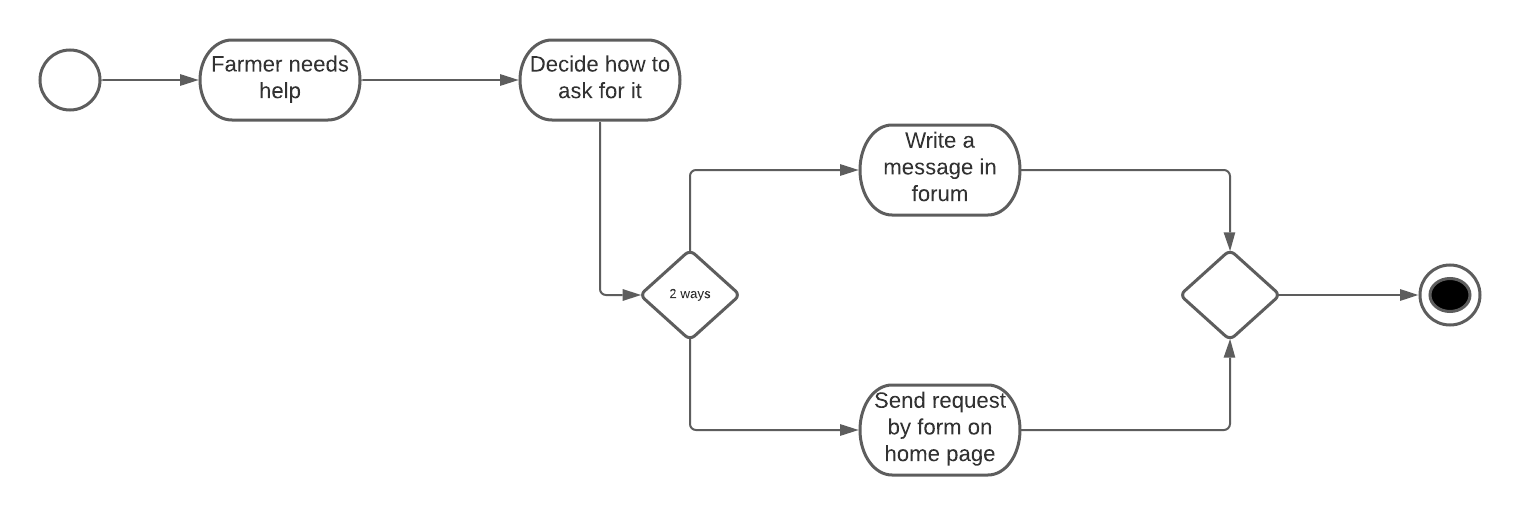
\includegraphics[width=1\textwidth]{images/State chart 3.png}
    \caption{Request of help.}
    \label{fig:state3}
    \end{center}
\end{figure}
\newpage
\subsection{Product Functions}
\label{subsection:2.2}
This section provides a summary of the main features and 
functions offered by the software regarding
the goals already described in section ~\ref{section:1.1.1}

In the following description it is important to highlight that both
the policy makers and the farmers must be logged in.

\subsubsection{Farmers insert data} 
This functionality is accessible to all farmers. 
The application provides a form in which the farmer can easily insert data of his/her production.
The form is easy to fill in, in order to complete it the farmer need to indicate:
\begin{itemize}
    \item the \textbf{type of product}
    \item the \textbf{amount} producted of the selected type
    \item the \textbf{date} relative to the date of the production
\end{itemize}
If the farmer needs to add more than one type of product, 
he/she can fill in the form multiple times.
After completing the form the user is redirected to the homepage and the policy makers 
can see the updated data.
This functionality can be done more than once a day since the farmer can select the date, 
so it is possible for him to insert data of past days too.
This operation can be repeated more than once a day since the farmer can select the date, so it is possible for him/her to insert data of past days too.



\subsubsection{Farmers visualize data}
This functionality lets the farmer visualize all the data 
acquired from the system. The farmer can visualize all data on his homepage.\\
The application shows:
\begin{itemize}
    \item meteorological  short-term and long-term forecast
    \item amount of water used by the farmer
    \item humidity of soil 
    \item personalized suggestions concerning specific crops to plant or specific 
    fertilizers to use – based on their location and type of production
\end{itemize}

\textbf{Should I say why he needs to visualize this data or how he uses it}


This functionality is always up to date, and does not need 
any input from the farmer.
It is used by the farmer only to have a general view of 
his farm and on how he could improve the productivity of his farm.



\subsubsection{Identify how farmers are performing}
The main features of the policy makers is to evaluate the work of each Farmer. 
In order to do that, they periodically analyze each farm page: 
the system allows them to visualize all the data in those pages 
(but not to modify it).
The analysis takes place twice a month.
With this analysis they classify the workers in two different way:
\begin{itemize}
    \item GOOD farmer : those how have been able to produce a significant amount of product with low resources, despite bad weather in that period.
    \item BAD farmer : those who did not produce much.
\end{itemize}
Policy makers inform each farmer the result they have achieved with a notification: 
\begin{itemize}
    \item GOOD farmers receive a special 
    incentive, and also a request to submit 
    from their personal web page some advice that could be useful to the others. 
    \item To BAD farmers is asked to submit an explicit request of help specifying the problems they had.
\end{itemize}
The system has a specific web page that allows all 
the users to look at a map of the area in which are 
specified all the farms. It is also shown if the farm's owner has performed 
a good job in that period.
At the end of each analysis the policy makers 
update the map (they are the only ones that are able to modify it).



\subsubsection{Interaction between farmers}
This functionality permits the farmers to comunicate with each other. 
The application has a specific web page were the farmers can send messages 
whenever they want.
If a farmer has an issue, before submitting a formal request of help to 
the policy makers 
by their home page, he can ask informally an advice by sending a message 
in the Forum.
It is not necessary to be a good farmer in order to answer someone elses 
message. All the messages are visible to everyone and 24h. 
Since it is an online application an internet connection is required to read or write 
on this page.



\subsection{Scenarios}
\subsubsection{Scenario 1}


\subsection{User Characteristics}
Dream has two different customers that need to be 
distinguished in order to provide the various 
features specified in subsection ~\ref{subsection:2.2}.
\subsubsection{Farmer}
- Can register on Dream in order to be recognized as farmer.\\
- Must log in on the website to use the services offered.\\
- Can discuss with other farmers.\\
- Is able to insert data about their daily production. \\
- Can ask for help to other farmers or to policy makers.\\
- Can retrieve data regarding weather forecast, water irrigation system or humidity of soil.\\
- Can look for advice of several products.\\
- Can check whether their performance is identified as good or bad.
\subsubsection{Policy Maker}
- Already has the credential to access to the system.\\
- Must login to Dream to benefit of its services.\\
- Can look all farms' pages.\\
- Can update the map.\\
- Can send suggestions to whom explicitly notices a problem.\\
- Can send notifications to the farmers.\\
- Decides the value of the incentive for the good farmers.\\
- Evaluates the performance of the farmers.\\



\subsection{Domain Assumptions, Dependencies and Constraints}
This subsection focuses on what it is assumed in order for our system to offer the services as expected.
Moreover it focuses on the limitations that the system could face.

\subsubsection{Domain Assumptions}
\textbf{DA1} In order to access the system users need to have Internet connection.\\
\textbf{DA2} Farmers always insert correct data on their production activity.\\
\textbf{DA3} Data from sensors is always correct.\\
\textbf{DA4} Date and Time on the system are always correct.\\
\textbf{DA5} The position of the Farm is always correct.\\
\textbf{DA6} Internet connection works always without errors.\\
\textbf{DA7} Meteorological data is accurate.\\
\textbf{DA8} Every farm has a different position.\\
\textbf{DA9} Each farm belongs to exacly one farmer.\\
\textbf{DA10} Discussion on the forum are related only to the farm activity.\\
\textbf{DA11} Formal request of help must be related to a farmer's own production.\\
\textbf{DA12} Advice on a product must be given by a farmer that produces the same type.\\
\textbf{DA13} Performances of farmers are always identified correctly.\\
\textbf{DA14} Farmers can insert data more than once a day.\\
\textbf{DA15 The username must be unique.}\\
\textbf{DA16} Policy Makers have a given username and password to access the system.

\subsubsection{Constraints}


\section{Specific Requirements}
\subsubsection{External Interface Requirements}

\subsubsection{User Interfaces}
qui ci vanno tutti i mockups con descrizione

\subsubsection{Hardware Interfaces}
The application does not need any specific hardware requirements. 

\subsubsection{Software Interfaces}
The web app requires a computer with a web browser installed and connected to 
The system has to rely on a DBMS API. It allows the management of all the data the system 
needs in order to provide its functionalities, described in subsection ~\ref{subsection:2.2}.

\subsubsection{Communication Interfaces}
All the communications between users and Dream website are made via HTTPS.

\newpage

\subsection{Functional Requirements}
\subsubsection{Use Case Diagram}
\subsubsection{Use Cases Description ad Sequence Diagram}
\begin{enumerate}
    \item \textbf{Farmer Registration} 
        \begin{longtable}{p{0.26\linewidth}p{0.75\linewidth}}
            \toprule
            \textbf{Name} & \textbf{Farmer Registration} \\
            \midrule
            \textbf{Actors} & Farmer \\
            \midrule
            \textbf{Entry conditions} & The web application has started\\
            \midrule
            \textbf{Flow of events} & 
            \begin{enumerate}
                \item The farmer wants to sign up
                \item The farmer inserts email, name, password, farm's name and farm's position 
                \item The farmer clicks submit
                \item The system checks if email is unique and if all the form is correctly fill up 
                \item The system inserts the information in the data base
            \end{enumerate} \\
            \midrule
            \textbf{Exit conditions} & The farmer is signed up\\
            \midrule
            \textbf{Exceptions} & 
            \begin{itemize}
                \item If the farmer did not insert data correctly the system will send an alert and let the user do that again
                \item If the email is already present in the database the system will send an alert saying that the email already exists
            \end{itemize} \\
            \bottomrule
            \caption{\emph{Farmer Registration} use case description}
        \end{longtable}
        
            \begin{figure}[H]
                \begin{center}
                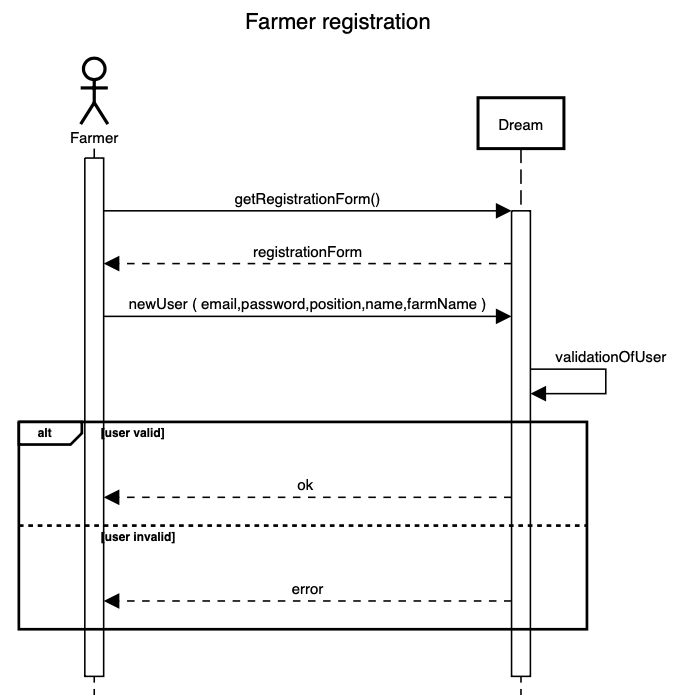
\includegraphics[width=0.7\textwidth]{sequence/FarmerRegistration.png}
                \caption{\emph{Farmer Registration} sequence diagram}
                \label{fig:sequence1}
                \end{center}
            \end{figure}

        \item \textbf{Farmer Login}
        \begin{longtable}{p{0.26\linewidth}p{0.75\linewidth}}
            \toprule
            \textbf{Name} & \textbf{Farmer Login} \\
            \midrule
            \textbf{Actors} & Farmer \\
            \midrule
            \textbf{Entry conditions} & The web application has started\\
            \midrule
            \textbf{Flow of events} & 
            \begin{enumerate}
                \item The farmer wants to log in
                \item The farmer inserts email and password
                \item The farmer clicks submit
                \item The system checks if the credentials are correct
                \item The system notifies the farmer about the correct login
            \end{enumerate} \\
            \midrule
            \textbf{Exit conditions} & The farmer has logged in\\
            \midrule
            \textbf{Exceptions} & 
            \begin{itemize}
                \item If the system does not recognize the email it will send and alert to the farmer saying that the email inserted is wrong
                \item If the password is not correct the system will notify the farmer
            \end{itemize} \\
            \bottomrule
            \caption{\emph{Farmer Login} use case description}
        \end{longtable}
        
        \begin{figure}[H]
        \begin{center}
        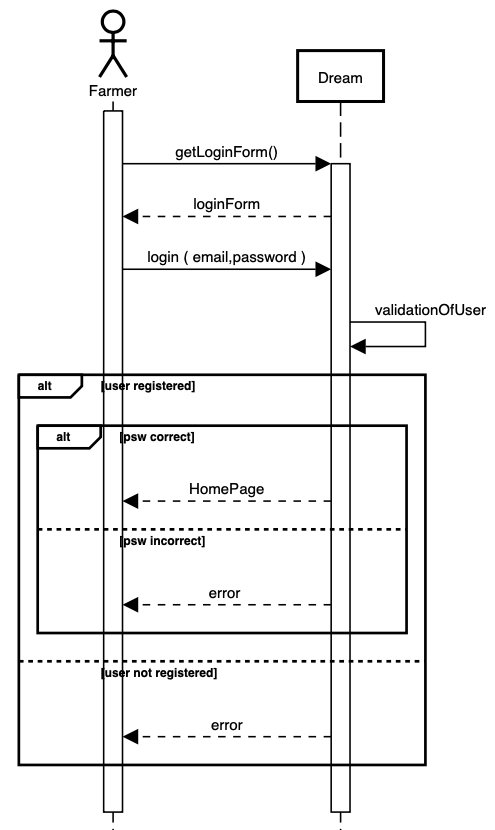
\includegraphics[width=0.5\textwidth]{sequence/FarmerLogin.png}
        \caption{\emph{Farmer Login} sequence diagram}
        \label{fig:sequence2}
        \end{center}
        \end{figure}


        \item Farmer send a message on the Forum
        \item \begin{longtable}{p{0.26\linewidth}p{0.75\linewidth}}
            \toprule
            \textbf{Name} & \textbf{Farmer sends a message on the forum} \\
            \midrule
            \textbf{Actors} & Farmer \\
            \midrule
            \textbf{Entry conditions} & The farmer has logged in\\
            \midrule
            \textbf{Flow of events} & 
            \begin{enumerate}
                \item The farmer wants to send a message
                \item The farmer clicks on forum button
                \item The system send the ser to the forum page
                \item The farmer inserts the message 
                \item The farmer clicks on send message
                \item The system inserts the message into the database 
            \end{enumerate} \\
            \midrule
            \textbf{Exit conditions} & The farmer's message is published\\
            \midrule
            \textbf{Exceptions} & 
            \begin{itemize}
                \item If the message body is empty the system shows an error alert
            \end{itemize} \\
            \bottomrule
            \caption{\emph{Farmer message} use case description}
        \end{longtable}
        \begin{figure}[H]
            \begin{center}
            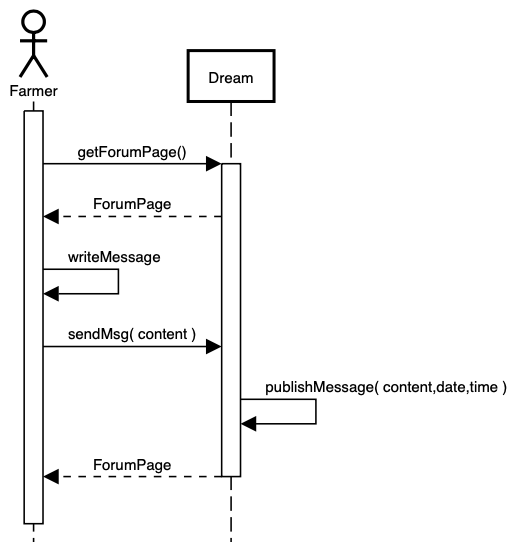
\includegraphics[width=0.6\textwidth]{sequence/messageOnForum.png}
            \caption{\emph{Farmer message} sequence diagram}
            \label{fig:sequence3}
        \end{center}
        \end{figure}

    \item Find a farmer on the Map\\
    \textbf{the farmers can only see the map with all the farm's, not if one is good or bad!}
    \begin{figure}[H]
        \begin{center}
        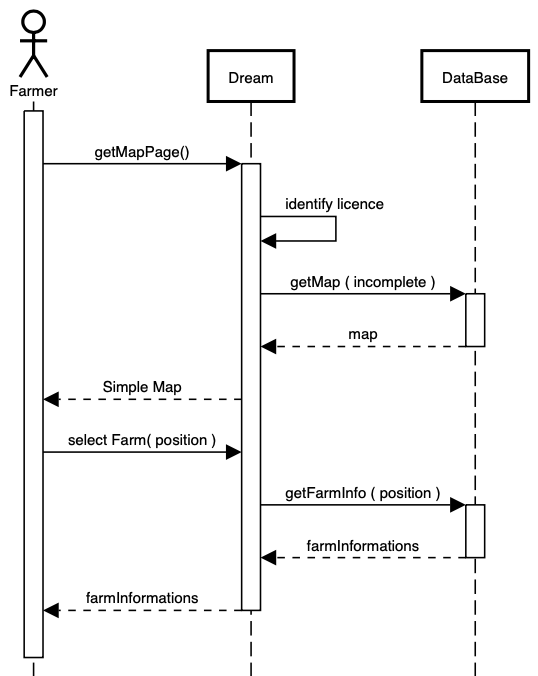
\includegraphics[width=0.7\textwidth]{sequence/VisializeMap.png}
        \caption{Find a farmer on the Map.}
        \label{fig:state4}
        \end{center}
    \end{figure}
    
    \item Find farm’s information
    \begin{figure}[H]
        \begin{center}
        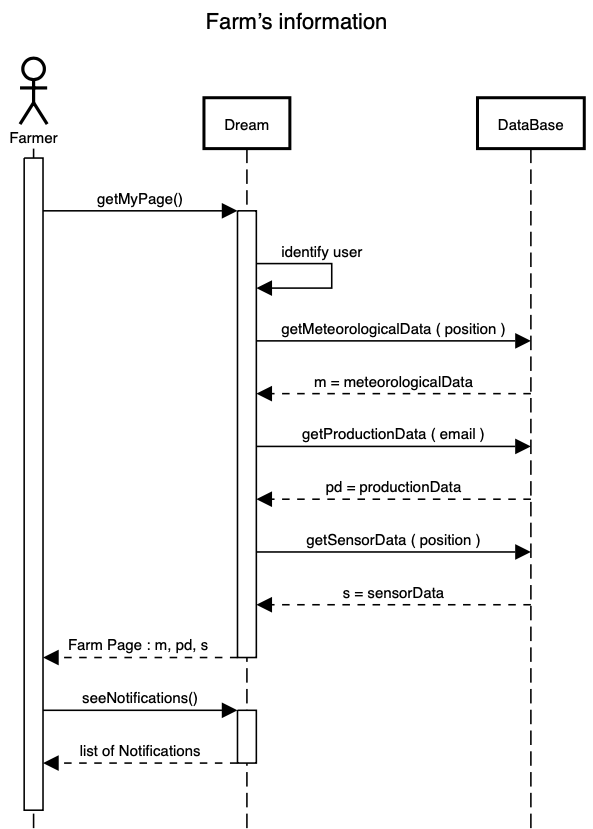
\includegraphics[width=0.7\textwidth]{sequence/FarmInformation.png}
        \caption{Find farm’s information.}
        \label{fig:state5}
        \end{center}
    \end{figure}
    \item Submit a request of help\\
    \textbf{I put only the case of a forml request to the Policy Maker (button on Farm Page) if you want we can create 2 "secion" (alt) one with this formal request and one sending a message on Forum (but is yet specified in 3)}
    \begin{figure}[H]
        \begin{center}
        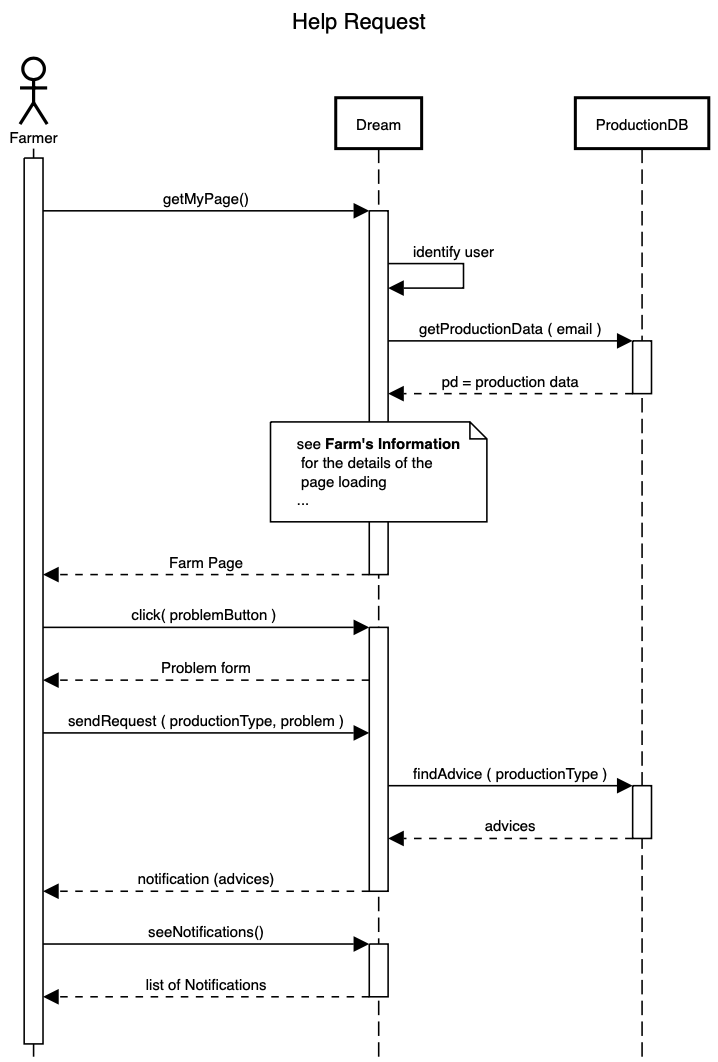
\includegraphics[width=0.7\textwidth]{sequence/HelpRequest.png}
        \caption{Submit a request of help.}
        \label{fig:state6}
        \end{center}
    \end{figure}
    \item Submit an advice
    \begin{figure}[H]
        \begin{center}
        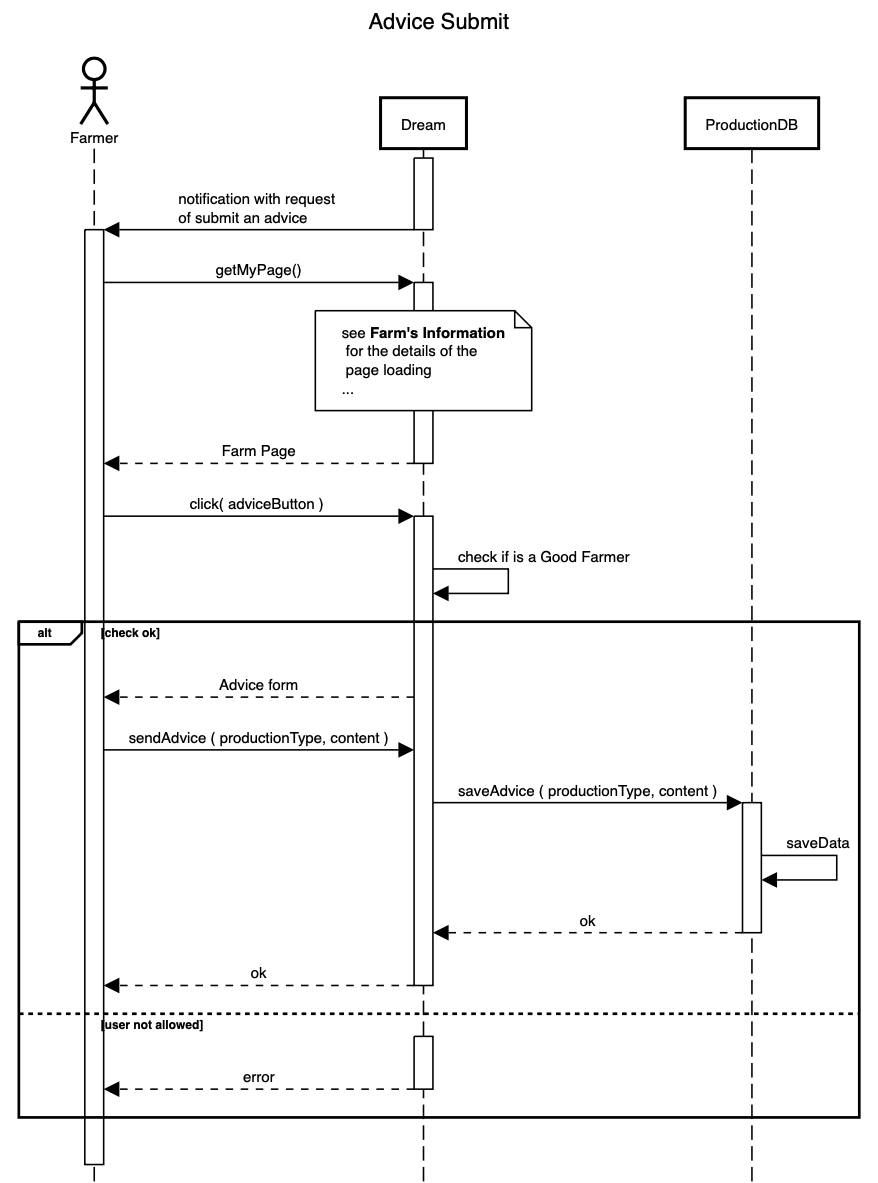
\includegraphics[width=0.7\textwidth]{sequence/AdviceSubmit.png}
        \caption{Submit an advice.}
        \label{fig:state7}
        \end{center}
    \end{figure}
    \item Visualize notifications
    \begin{figure}[H]
        \begin{center}
        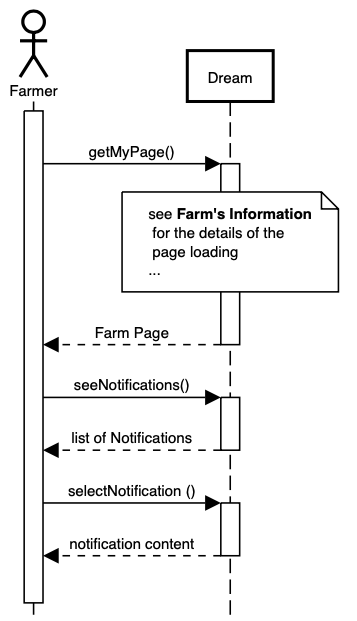
\includegraphics[width=0.7\textwidth]{sequence/SeeNotifications.png}
        \caption{Visualize notifications.}
        \label{fig:state8}
        \end{center}
    \end{figure}
    \item Policy Maker login
    \begin{figure}[H]
        \begin{center}
        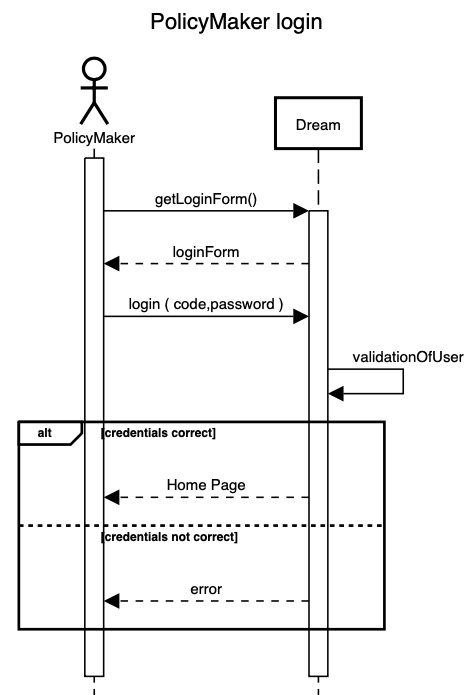
\includegraphics[width=0.7\textwidth]{sequence/PolicyMakerLogin.png}
        \caption{Policy Maker login.}
        \label{fig:state9}
        \end{center}
    \end{figure}
    \item Find a farm's page
    \begin{figure}[H]
        \begin{center}
        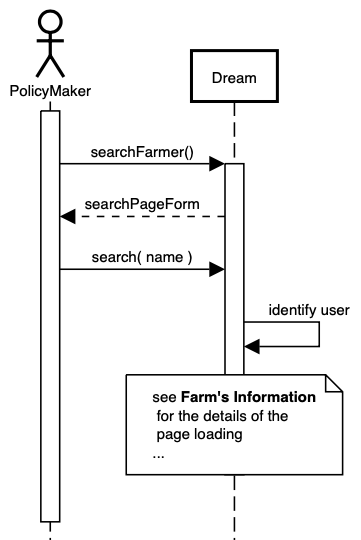
\includegraphics[width=0.7\textwidth]{sequence/PolicyMakerseachFarm.png}
        \caption{Find a farm's page.}
        \label{fig:state9}
        \end{center}
    \end{figure}
    \item Find a farmer on the Map
    \begin{figure}[H]
        \begin{center}
        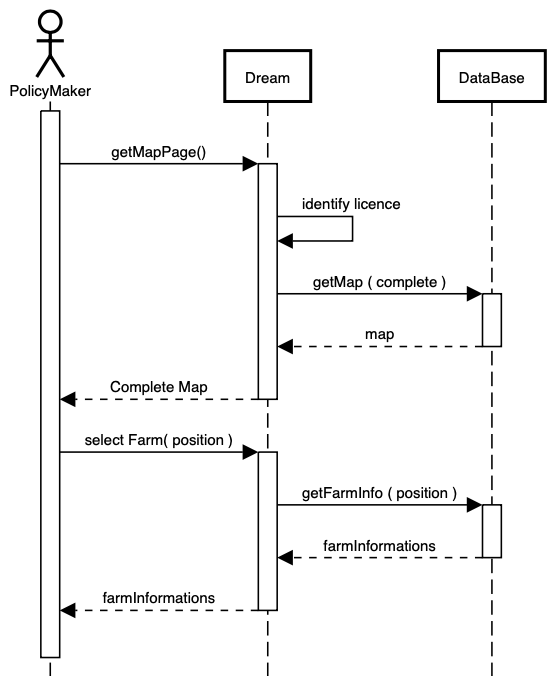
\includegraphics[width=0.7\textwidth]{sequence/searchOnMap.png}
        \caption{Find a farmer on the Map.}
        \label{fig:state9}
        \end{center}
    \end{figure}
    \item Update the Map
    \begin{figure}[H]
        \begin{center}
        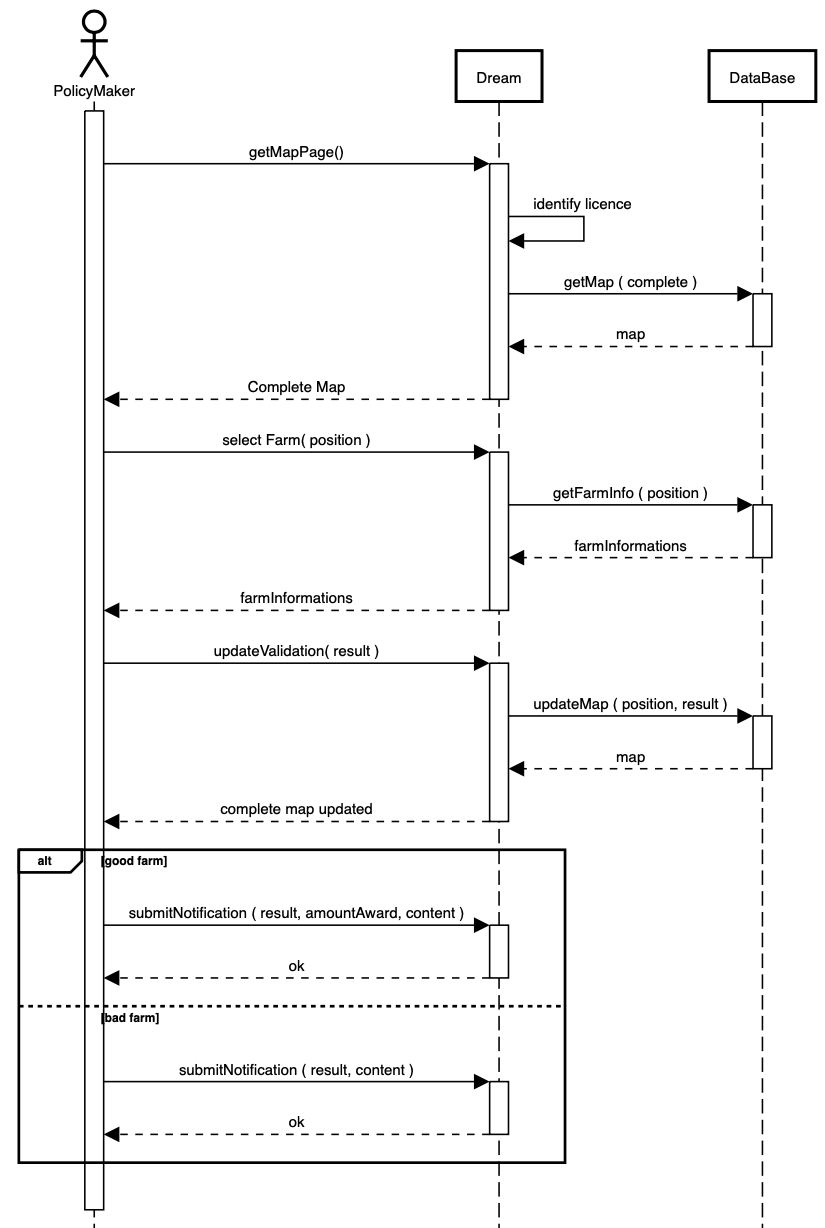
\includegraphics[width=0.7\textwidth]{sequence/updateMap.png}
        \caption{Update the Map.}
        \label{fig:state9}
        \end{center}
    \end{figure}
    \item Reply to a request of help
    \begin{figure}[H]
        \begin{center}
        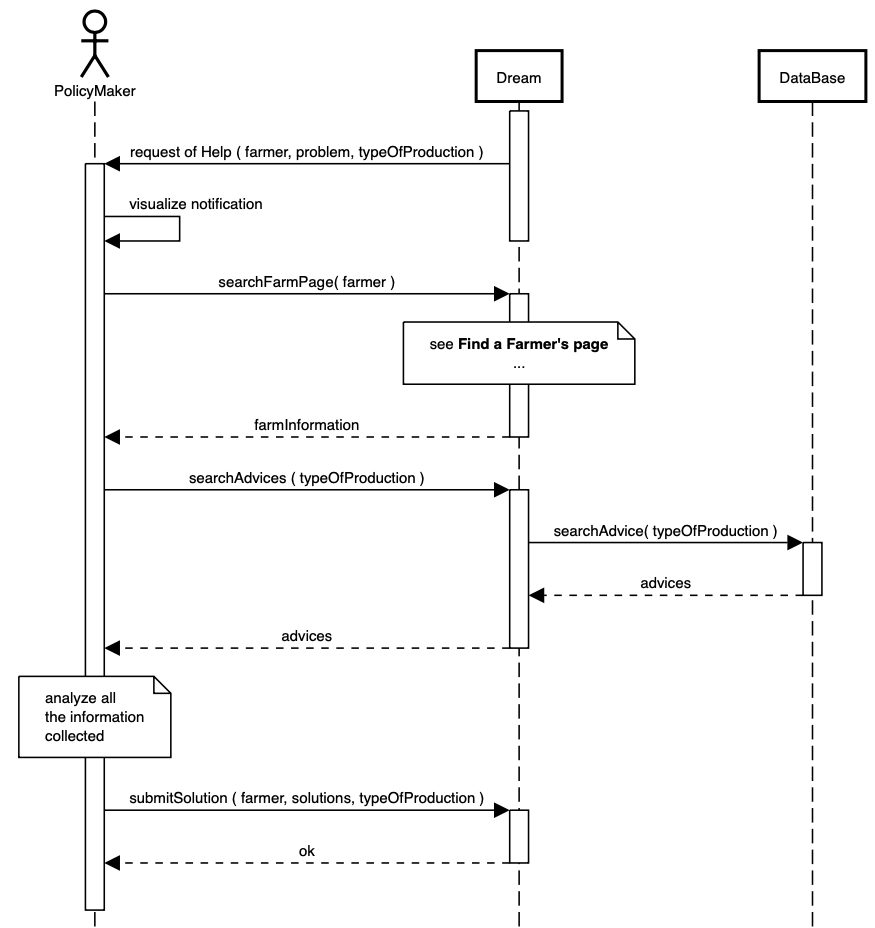
\includegraphics[width=0.7\textwidth]{sequence/replyHelp.png}
        \caption{Reply to a request of help.}
        \label{fig:state9}
        \end{center}
    \end{figure}
\end{enumerate}
\subsubsection{Scenarios}
\subsubsection{Requirements}
\textbf{R1} the system must allow farmers to register\\
\textbf{R2} the system must allow farmers to log in\\
\textbf{R3} the system must save the farmers registration data\\
\textbf{R4} the system must guarantee that each email address is unique\\
\textbf{R5} the system must verify that the email address is valid (the type!)\\
\textbf{R6} the system must save the farmers information about their production submitted\\
\textbf{R7} the system must allow farmers to insert the type of production \\
\textbf{R8} the system must allow farmers to insert the amount of production type\\
\textbf{R9} the system must allow farmers to specify a problem they faced to the Policy Makers\\
\textbf{R10} the system must allow farmers to select the type of production on which they had troubles\\
\textbf{R11} the system must save the advice submitted by the farmers\\
\textbf{R12} the system must allow farmers to select the type of product in their suggestion\\
\textbf{R13} the system must be able to show to the farmers advices send by the Policy Makers (as a notification)\\
\textbf{R14} the system must be able to show the meteorological data of the Farm’s position\\
\textbf{R15} the system must be able to show the farm’s sensor data \\
\textbf{R16} the system must allow farmers to send messages on the forum\\
\textbf{R17} the system must register date and time of a message in the forum\\
\textbf{R18} the system must be able to show all the messages on the forum\\
\textbf{R19} the system must be able to show the map of the zone\\
\textbf{R20} the system must be able to show the farms position on the map\\
\textbf{R21} the system must be able to show on the map if a farm is performing well or not \\
\textbf{R22} the system must allow farmers to visualise notification send by Policy Makers\\
\textbf{R23} the system does not allow Policy Makers to register\\
\textbf{R24} the system must allow Policy Makers to log in\\
\textbf{R25} the system must allow Policy Makers to search a farm by name (OK?)\\
\textbf{R26} the system must allow Policy Makers to see all farms’ pages\\
\textbf{R27} the system must not allow Policy Makers to modify any farm’s page\\
\textbf{R28} the system must allow Policy Makers to update the performance of a farmer\\
\textbf{R29} the system must allow Policy Makers to send notification to the farmers\\
\textbf{R30} the system must allow Policy Makers to receive request of help by the farmers\\
\subsubsection{Traceability Matrix}

\subsection{Performance Requirements}
The system serves its user with a web application. All the computations will take place on the server side, 
thus the app is meant to be lightweighted. Moreover the load in the night is expected to be really low.
There are no problems about reliability. The insertion of new data requires a quick response in order to store 
it in the system.

\subsection{Design Constraints}
\subsubsection{Standards Compliance}
The only standard that needs to be highlighted here is the interaction with the database. It is important that the information are stored 
in a standardized form. In such manner, it is easier to memorize and retrieve data.


\subsubsection{Any Other Constraints}
Interaction between Dream and users needs to consider also regulatory policies.
As a matter of fact the application asks and retrieves data of each farmer.
More information about security and privacy will be provided in the section~\ref{subsubsection:3.4.3}


\subsection{Software System Attributes}

\subsubsection{Reliability}
The system must prevent any failure in order to guarantee continuity. 
Simultaneous accesses are expected to work, especially in the afternoon when users are expectd to insrt and retrieve more information.

\subsubsection{Availability}
It is expected that the system has the lowest downtime possible. 
The system is available with a minimum time of 96\%, 
so that it about 14 days a year of downtime are allowed.


\subsubsection{Security}
\label{subsubsection:3.4.3}
Security of the data and of the communication user-system is a primary concern. Users credential are stored in a data base, so the system crypt the password data before store it. The system recognises the right type of user during the log in phase to ensure providing the correct level visibility of the data and the permission to update them or not. In this way farmer’s privacy is guaranteed. As a matter of fact a farmer can’t see another farmer’s page.


\subsubsection{Maintanability}
The web application requires ordinary maintenance for improvements and in order to fix potential bugs. 
It is going to be scheduled at local night time, when user traffic is the lowest.
Moreover the system must be designed in a way that allows future addition of features.

\subsubsection{Portability}
The system as a web application must run on different software system as Windows, Linux an macOS.
On the server side is crucial focusing on the interaction between APIs and the data base to insert, update or read data.



\section{Formal Analysis using Alloy}

\section{Effort Spent}

\end{document}
